\chapter{Control de motores GIM8108v3}

\thispagestyle{plain}
\renewcommand{\tablename}{Tabla}

\section{Introducción}

En este capítulo se desarrollarán los distintos pasos seguidos en el desarrollo de este apartado del trabajo de fin de grado. Para ello, se empezó estudiando el firmware de los motores para determinar su funcionamiento y método de comunicación, con el fin de modelarlo posteriormente en Simulink

\section{Firmware 1.9}

Para entender como funciona el empaquetado y desempaquetado de mensajes CAN se utiliza el archivo proporcionado por el fabricante sobre el driver del motor \cite{Katz2021}. En el archivo se enlaza un ejemplo de comunicación con el motor realizado por Ben Katz. A partir del código main.cpp se encuentra cómo se interpreta el mensaje CAN y cuáles son los parámetros que requiere el motor para funcionar. Véase el fragmento de código 4.1.

\begin{lstlisting}[language=Arduino, caption= main.cpp, basicstyle=\scriptsize]
/// Value Limits ///
    #define P_MIN -12.5f
    #define P_MAX 12.5f
    #define V_MIN -45.0f
    #define V_MAX 45.0f
    #define KP_MIN 0.0f
    #define KP_MAX 500.0f
    #define KD_MIN 0.0f
    #define KD_MAX 5.0f
    #define T_MIN -18.0f
    #define T_MAX 18.0f

/// CAN Command Packet Structure ///
/// 16 bit position command, between -4*pi and 4*pi
/// 12 bit velocity command, between -30 and + 30 rad/s
/// 12 bit kp, between 0 and 500 N-m/rad
/// 12 bit kd, between 0 and 100 N-m*s/rad
/// 12 bit feed forward torque, between -18 and 18 N-m
/// CAN Packet is 8 8-bit words
/// Formatted as follows.  For each quantity, bit 0 is LSB
/// 0: [position[15-8]]
/// 1: [position[7-0]] 
/// 2: [velocity[11-4]]
/// 3: [velocity[3-0], kp[11-8]]
/// 4: [kp[7-0]]
/// 5: [kd[11-4]]
/// 6: [kd[3-0], torque[11-8]]
/// 7: [torque[7-0]]
 
void pack_cmd(CANMessage * msg, float p_des, float v_des, float kp, float kd, float t_ff){
     /// limit data to be within bounds ///
     p_des = fminf(fmaxf(P_MIN, p_des), P_MAX);                    
     v_des = fminf(fmaxf(V_MIN, v_des), V_MAX);
     kp = fminf(fmaxf(KP_MIN, kp), KP_MAX);
     kd = fminf(fmaxf(KD_MIN, kd), KD_MAX);
     t_ff = fminf(fmaxf(T_MIN, t_ff), T_MAX);
     /// convert floats to unsigned ints ///
     int p_int = float_to_uint(p_des, P_MIN, P_MAX, 16);            
     int v_int = float_to_uint(v_des, V_MIN, V_MAX, 12);
     int kp_int = float_to_uint(kp, KP_MIN, KP_MAX, 12);
     int kd_int = float_to_uint(kd, KD_MIN, KD_MAX, 12);
     int t_int = float_to_uint(t_ff, T_MIN, T_MAX, 12);
     /// pack ints into the can buffer ///
     msg->data[0] = p_int>>8;                                       
     msg->data[1] = p_int&0xFF;
     msg->data[2] = v_int>>4;
     msg->data[3] = ((v_int&0xF)<<4)|(kp_int>>8);
     msg->data[4] = kp_int&0xFF;
     msg->data[5] = kd_int>>4;
     msg->data[6] = ((kd_int&0xF)<<4)|(t_int>>8);
     msg->data[7] = t_int&0xff;
     }
      
/// CAN Reply Packet Structure ///
/// 16 bit position, between -4*pi and 4*pi
/// 12 bit velocity, between -30 and + 30 rad/s
/// 12 bit current, between -40 and 40;
/// CAN Packet is 5 8-bit words
/// Formatted as follows.  For each quantity, bit 0 is LSB
/// 0: [position[15-8]]
/// 1: [position[7-0]] 
/// 2: [velocity[11-4]]
/// 3: [velocity[3-0], current[11-8]]
/// 4: [current[7-0]]

void unpack_reply(CANMessage msg){
    /// unpack ints from can buffer ///
    int id = msg.data[0];
    int p_int = (msg.data[1]<<8)|msg.data[2];
    int v_int = (msg.data[3]<<4)|(msg.data[4]>>4);
    int i_int = ((msg.data[4]&0xF)<<8)|msg.data[5];
    /// convert ints to floats ///
    float p = uint_to_float(p_int, P_MIN, P_MAX, 16);
    float v = uint_to_float(v_int, V_MIN, V_MAX, 12);
    float i = uint_to_float(i_int, -I_MAX, I_MAX, 12);
     
    if(id == 2){
        theta1 = p;
        dtheta1 = v;
        }
    else if(id ==3){
        theta2 = p;
        dtheta2 = v;
        }
    
    //printf("%d  %.3f   %.3f   %.3f\n\r", id, p, v, i);
    } 
     
\end{lstlisting}

En las primeras líneas se definen los valores máximos y mínimos de los parámetros del motor. En el caso del motor utilizado en este proyecto, estos parámetros varían ligeramente.

\begin{itemize}
    \item Posición: En el firmware sus límites están en \(-12.5\ rad\) y \(12.5\ rad\) aunque los motores de SteadyWin funcionan entre \(-95\ rad\) y \(95\ rad\).
    \item Velocidad: Comprendida entre \(-45\ rad/s\) y \(45\ rad/s\).
    \item Kp: Con valores de \(0\) a \(500\ N-m/rad\)
    \item Kd: Sus límites están entre \(0\) y \(5\ N-m\cdot s/rad\)
    \item Torque: Comprendido entre \(-18\ N\cdot m\) y \(18\ N\cdot m\).
\end{itemize}

Los valores de estos parámetros condicionarán el controlador que ejecutará el motor. Diferenciando:

\begin{itemize}
    \item Control de Posición: Se encarga de mantener la posición del motor. En este caso influye los parámetros Posición, Velocidad, Kp y Kd.
    \item Control de Velocidad: Este se encargará de mantener una velocidad constante. Los parámetros modificables en este caso son Kd y Velocidad.
    \item Control de Torque: No se utiliza en este proyecto. Cabe destacar que este tipo de control permite mantener una velocidad constante incluso cuando la carga varía.
\end{itemize}

Posteriormente, se declaran las funciones \textit{unpack\_reply} y \textit{pack\_cmd}, encargadas del empaquetado y desempaquetado de los mensajes CAN.

\begin{itemize}
    \item \textit{pack\_cmd}: Encargada de empaquetar el mensaje CAN que se enviará al motor. \(8\ bytes\) de información que incluyen Posición, Velocidad, Kp, Kd y Torque. 
    \item \textit{unpack\_reply}: Se encarga del desempaquetado del mensaje CAN recibido. Este tendrá un tamaño de \(5\ bytes\), en los que se almacena Posición, Velocidad y Corriente. 
\end{itemize}

\section{Modelo Simulink}
\subsection{Bloques CAN}
Haciendo uso del paquete \textit{Vehicle Network Toolbox} de MATLAB y Simulink, se añaden al modelo los bloques \textit{CAN Pack} y \textit{CAN Unpack}. 

\begin{figure}[H]
    \centering
    \begin{subfigure}[b]{0.45\textwidth}
        \centering
        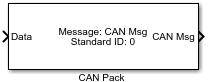
\includegraphics[width = \textwidth]{imagenes/CAN Pack Block.png}
        \caption{CAN Pack \cite{CANPack-MathWorks}}
        \label{fig:CAN-Pack}
    \end{subfigure}
    \hfill
    \begin{subfigure}[b]{0.45\textwidth}
        \centering
        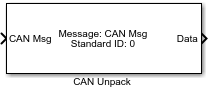
\includegraphics[width = \textwidth]{imagenes/CAN UnPack Block.png}
        \caption{CAN UnPack \cite{CANUnpack-MathWorks}}
        \label{fig:CAN-UnPack}
    \end{subfigure}
    \caption{Bloques CAN}
    \label{fig:BloquesCAN}
\end{figure}

\subsubsection{CAN Pack}
El bloque CAN Pack carga datos de señal en un mensaje CAN a intervalos específicos durante la simulación. Para poder configurar dicho bloque seleccionamos que \textit{Data input} sea \textit{manually specified signals}. Esto nos permitirá crear las señales específicas de nuestro motor. Este bloque también permite la entrada de estas especificaciones a través de archivos del tipo CANdb o ARXML. 


\begin{figure}[H]
    \centering
    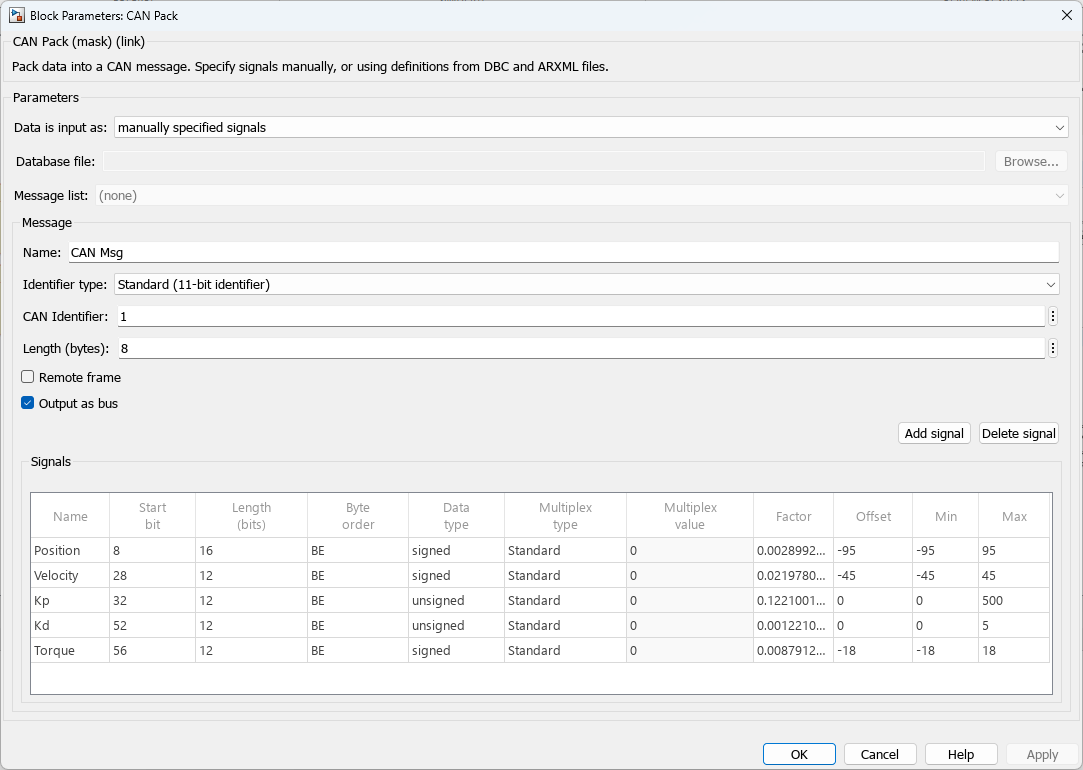
\includegraphics[width=1\linewidth]{imagenes/Simulink - CAN Pack.png}
    \caption{CAN Pack - Block Parameters}
    \label{fig:Simulink-CANPack}
\end{figure}

A partir de la información obtenida analizando el código 4.1, se concluye que \textit{Byte order} es \textit{BE (Big-Endian)} y \textit{Data type} es \textit{unsigned}. Los valores máximos y mínimos introducidos en esta tabla son los valores físicos. \textit{Factor} y \textit{Offset} se deben calcular para cada una de las señales. Utilizando la expresión proporcionada por MATLAB \cite{CANPack-MathWorks} :

\begin{equation}
    raw\_value = (physical\_value - Offset) / Factor
\end{equation}

Sabiendo que el valor mínimo de la señal corresponde a un valor \textit{raw} de '\(0\)' y el máximo a `\(2^{bits} - 1\)', se calculan los \textit{Factor} y \textit{Offset} para cada una de estas señales. 

\begin{lstlisting}[caption={Código de cálculo de Factor y Offset (CAN Pack) en MATLAB}, label={Código de cálculo de Factor y Offset (CAN Pack) en MATLAB}, basicstyle=\scriptsize]
% raw_value = (physical_value - Offset) / Factor

% ----- Position -----
syms Offset Factor;

Min = -95;
Max = 95;
bits = 16;

[Factor, Offset] = solve(0 == (Min - Offset) / Factor, 2^bits - 1 == (Max - Offset) / Factor, Factor, Offset);
Factor = vpa(Factor) % Aproximación de Factor
Offset

% ----- Velocity -----
syms Offset Factor;

Min = -45;
Max = 45;
bits = 12;

[Factor, Offset] = solve(0 == (Min - Offset) / Factor, 2^bits - 1 == (Max - Offset) / Factor, Factor, Offset);
Factor = vpa(Factor) % Aproximación de Factor
Offset

% ----- Kp -----
syms Offset Factor;

Min = 0;
Max = 500;
bits = 12;

[Factor, Offset] = solve(0 == (Min - Offset) / Factor, 2^bits - 1 == (Max - Offset) / Factor, Factor, Offset);
Factor = vpa(Factor) % Aproximación de Factor
Offset

% ----- Kd -----
syms Offset Factor;

Min = 0;
Max = 5;
bits = 12;

[Factor, Offset] = solve(0 == (Min - Offset) / Factor, 2^bits - 1 == (Max - Offset) / Factor, Factor, Offset);
Factor = vpa(Factor) % Aproximación de Factor
Offset

% ----- Torque -----
syms Offset Factor;

Min = -18;
Max = 18;
bits = 12;

[Factor, Offset] = solve(0 == (Min - Offset) / Factor, 2^bits - 1 == (Max - Offset) / Factor, Factor, Offset);
Factor = vpa(Factor) % Aproximación de Factor
Offset
\end{lstlisting}

Por último, sabiendo el orden que siguen los bits y su longitud, obtenemos la posición del bit de inicio de cada una.

\begin{figure}[H]
    \centering
    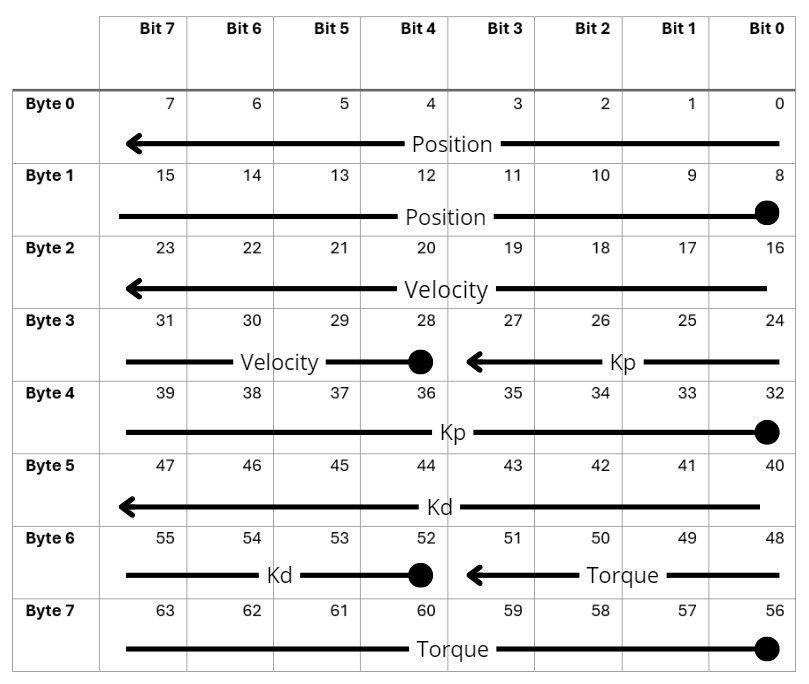
\includegraphics[width=0.75\linewidth]{imagenes/Simulink - CAN Pack - Start bit.png}
    \caption{Estructura del mensaje CAN enviado al motor.}
    \label{fig:Simulink-PackStartBit}
\end{figure}

\subsubsection{CAN Unpack}
El bloque CAN Unpack descomprime un mensaje CAN en datos de señal utilizando los parámetros de salida especificados. Estos datos se emiten como señales individuales. Para poder configurar dicho bloque seleccionamos que \textit{Data input} sea \textit{manually specified signals}. Esto nos va a permitir crear las señales específicas de nuestro motor. Este bloque, al igual que el de CAN Pack, permite la entrada de estas especificaciones a través de archivos del tipo CANdb o ARXML.

\begin{figure}[H]
    \centering
    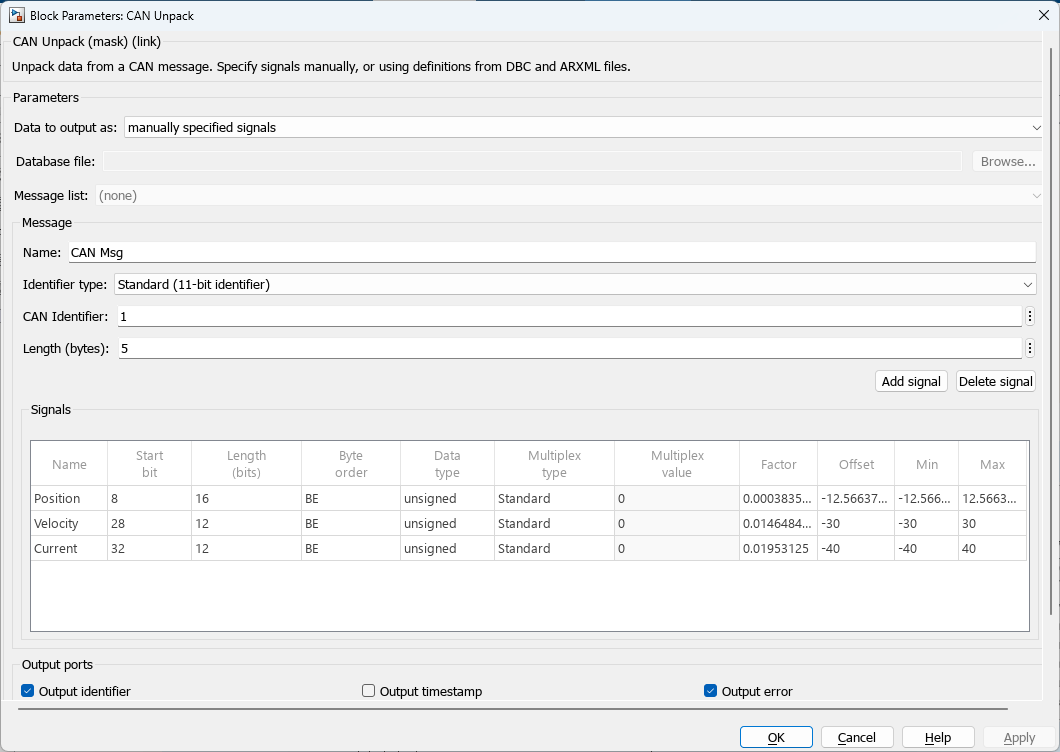
\includegraphics[width=1\linewidth]{imagenes/Simulink - CAN Unpack.png}
    \caption{CAN Unpack - Block Parameters}
    \label{fig:Simulink-CANUnpack}
\end{figure}

Observamos como el tamaño del mensaje enviado (\(5\ bytes\)) y recibido (\(8\ bytes\)) por el motor son distintos. El \textit{Byte order} sigue siendo del tipo \textit{BE} y \textit{Data type} \textit{unsigned}. Los valores máximos y mínimos que se introducen son los valores físicos. \textit{Factor} y \textit{Offset} se deben calcular nuevamente para cada una de las señales. Utilizando la expresión proporcionada por MATLAB \cite{CANUnpack-MathWorks} :

\begin{equation}
    physical\_value = raw\_value \times Factor + Offset 
\end{equation}

Sabiendo que el valor mínimo de la señal corresponde a un valor \textit{raw} de `\(0\)' y el máximo a `\(2^{bits} - 1\)', se calculan los \textit{Factor} y \textit{Offset} para cada una de estas señales. 

\begin{lstlisting}[caption={Código de cálculo de Factor y Offset (CAN UnPack) en MATLAB}, label={Codigo de calculo de Factor y Offset (CAN UnPack) en MATLAB}, basicstyle=\scriptsize]
% physical_value = raw_value * Factor + Offset

% ----- Position -----
syms Offset Factor;

Min = -4*pi;
Max = 4*pi;
bits = 16;

[Factor, Offset] = solve(Min == 0 * Factor + Offset, Max == (2^bits - 1) * Factor + Offset, Factor, Offset);
Factor = vpa(Factor) % Aproximación de Factor
Offset = vpa(Offset) % Aproximación de Offset

% ----- Velocity -----
syms Offset Factor;

Min = -30;
Max = 30;
bits = 12;

[Factor, Offset] = solve(Min == 0 * Factor + Offset, Max == (2^bits - 1) * Factor + Offset, Factor, Offset);
Factor = vpa(Factor) % Aproximación de Factor
Offset

% ----- Current -----
syms Offset Factor;

Min = -40;
Max = 40;
bits = 12;

[Factor, Offset] = solve(Min == 0 * Factor + Offset, Max == (2^bits - 1) * Factor + Offset, Factor, Offset);
Factor = vpa(Factor) % Aproximación de Factor
Offset

\end{lstlisting}

Por último, sabiendo el orden que siguen los bits y su longitud, obtenemos la posición del bit de inicio de cada una.

\begin{figure}[H]
    \centering
    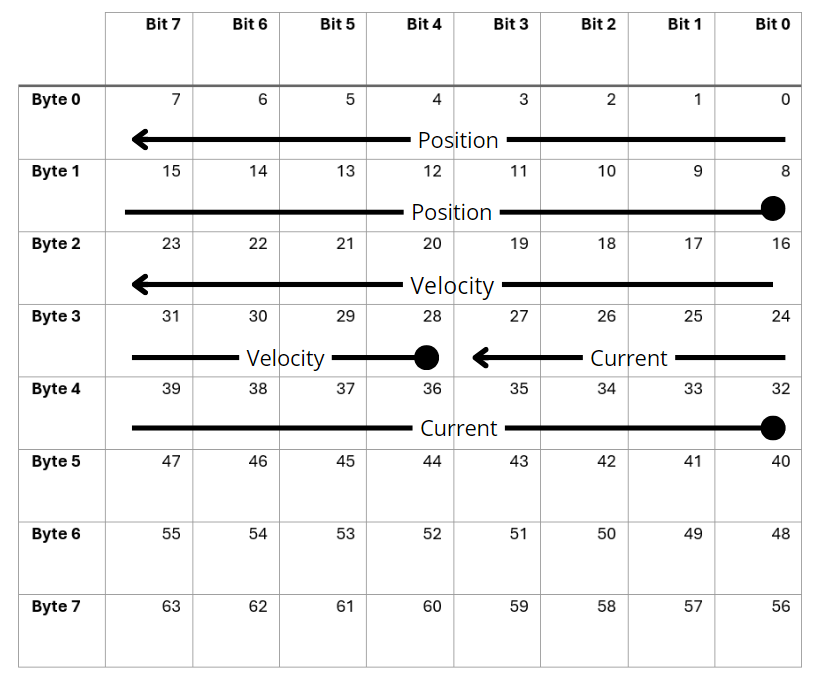
\includegraphics[width=0.75\linewidth]{imagenes/Simulink - CAN Unpack - Start bit.png}
    \caption{Estructura del mensaje CAN recibido desde el motor.}
    \label{fig:Simulink-UnpackStartbit}
\end{figure}

\subsection{Subsistema comunicación motores}

Los bloques configurados previamente serán aquellos que conformen la parte principal del subsistema `motores'. Este subsistema perteneciente al control del vehículo recibirá como entradas seis vectores, cada uno correspondiente a una rueda del robot, y una entrada del tipo \textit{int} con la que se controlará el modo de funcionamiento de estas.

Cada uno de los vectores estará conformado por Posición, Velocidad, Kp, Kd y Par de Torsión. Asimismo, se establecen tres modos de operación de los motores:

\begin{itemize}
    \item Modo 0: Apagados - En este modo los motores se encuentran apagados y por tanto no se tiene ningún tipo de control sobre los mismo.
    \item Modo 1: Encendidos - Este modo se mantendrá siempre y cuando los motores se encuentren encendidos y con una velocidad distinta de 0. Se empleará un control de velocidad cuyos parámetros modificables serán \textit{Velocity} y \textit{Kd}, permaneciendo los demás a 0.
    \item Modo 2: Actualizar la posición cero - Este modo de funcionamiento se activará de forma automática cuando el motor esté encendido y la velocidad de entrada sea 0. En este modo se pasará de un control de velocidad a uno de posición, de este modo se consigue que el vehículo se quede inmóvil independientemente del grado de inclinación de la superficie en la que se encuentre.
\end{itemize}

\begin{figure}[H]
    \centering
    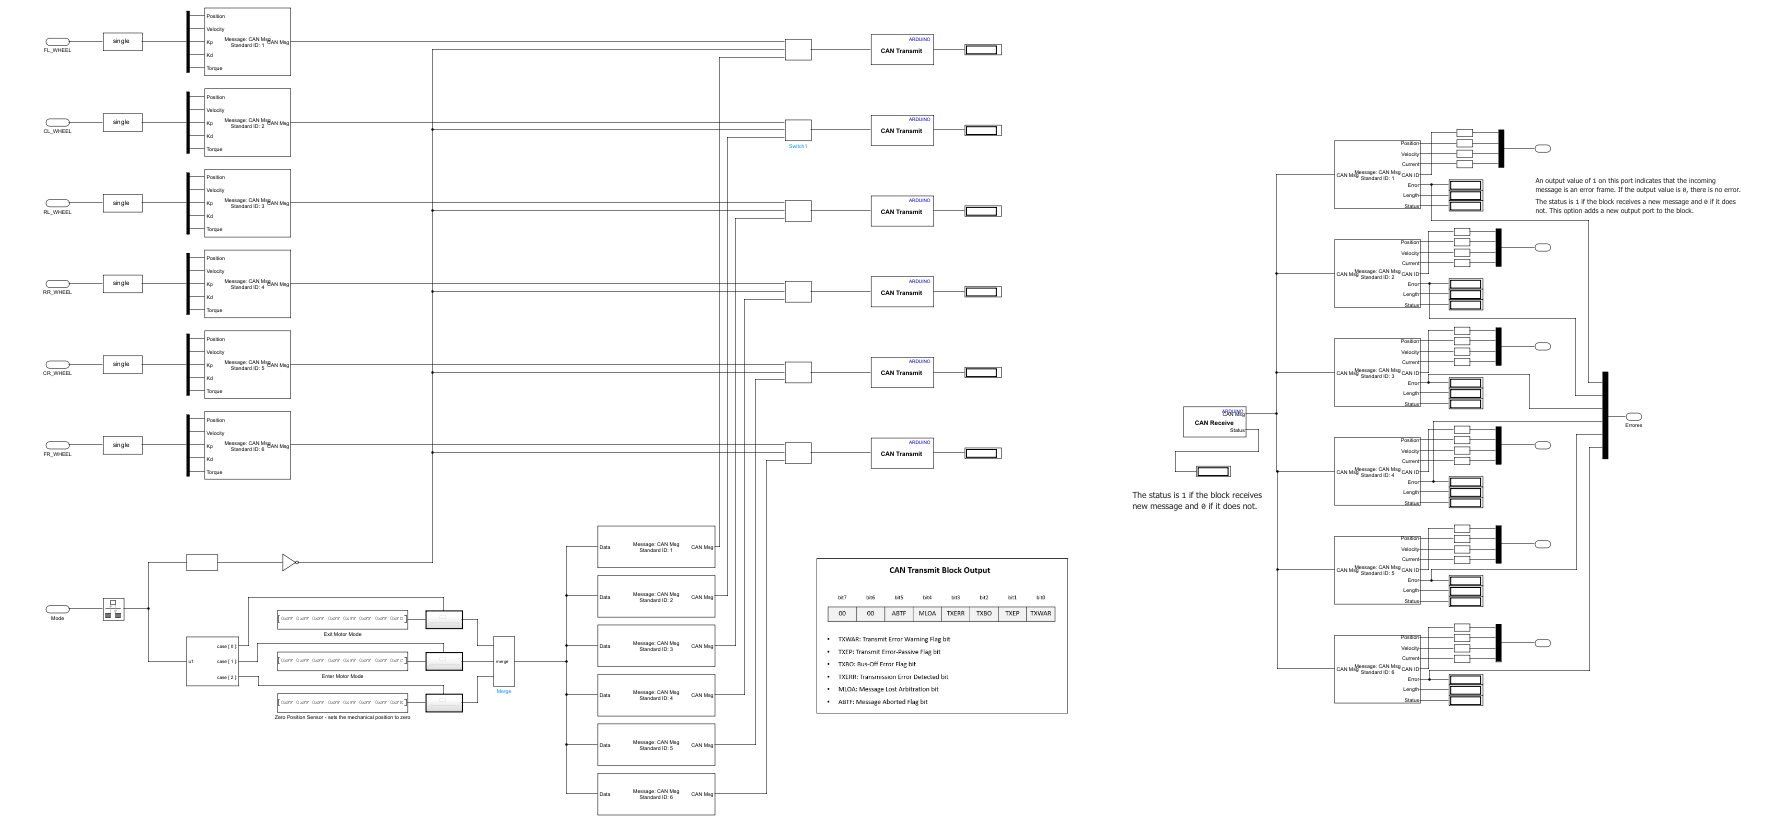
\includegraphics[width=1\linewidth]{imagenes/Simulink - Cont - General.png}
    \caption{Contenido del subsistema Motores.}
    \label{fig:Simulink-Motores}
\end{figure}

En este subsistema (Figura \ref{fig:Simulink-Motores}) se distinguen dos partes: transmisión a de información hacia los motores (Figura \ref{fig:Simulink-Motores1}) y recepción de datos desde estos.

\begin{figure}[H]
    \centering
    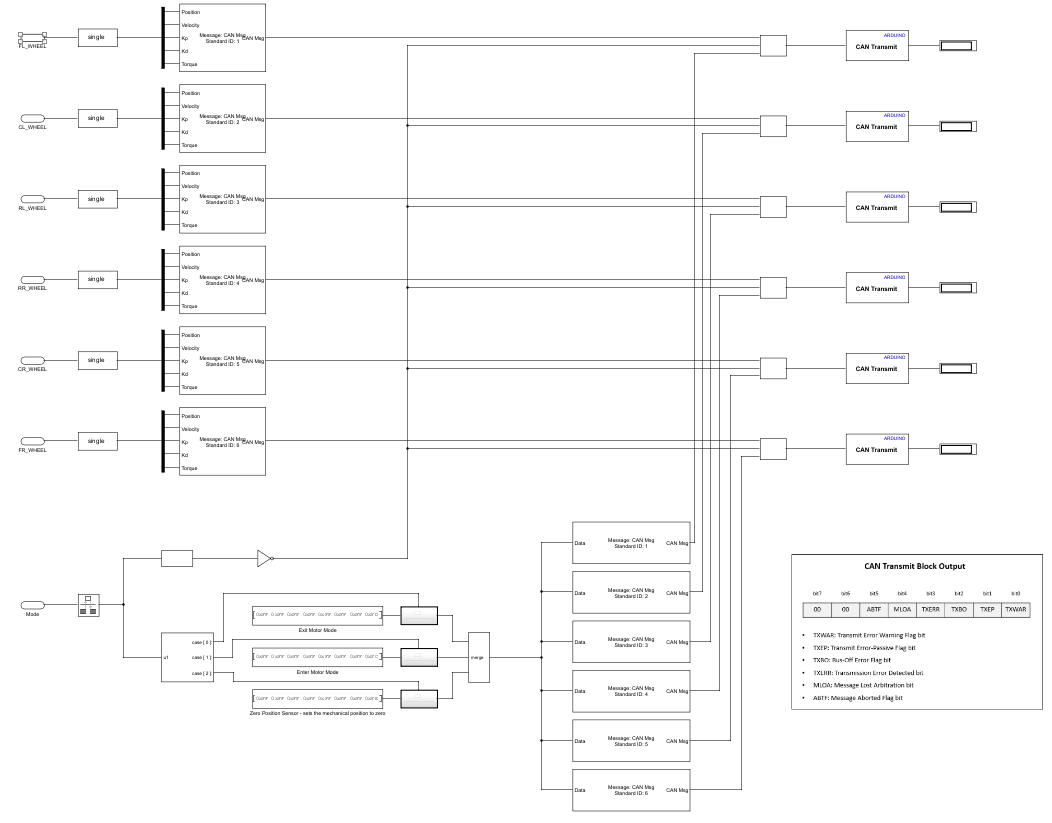
\includegraphics[width=1\linewidth]{imagenes/Simulink - Cont - 1.png}
    \caption{Transmisión de datos a los motores.}
    \label{fig:Simulink-Motores1}
\end{figure}


Esta primera parte recibe la entrada de `\textit{Mode}', que pasará por el bloque `\textit{Rate Transition}' (Figura \ref{fig:Rate Transition}) antes de utilizarse. Este bloque intermediario se encargará de manejar la transferencia de datos entre bloques que operan a diferentes velocidades. Se procederá a detectar los cambios de modo haciendo uso del bloque `\textit{Detect Change}' (Figura \ref{fig:Detect Change}). Este determinará si la señal de entrada que está recibiendo no es igual a la anterior. Teniendo que establecerse una condición inicial, que en este caso, será `0' puesto que los motores se encontraran inicialmente apagados. La salida de este bloque será un booleano con valor \textit{TRUE} si detecta cambio y \textit{FALSE} si no. 

\begin{figure}[H]
     \centering
     \begin{subfigure}[b]{0.45\textwidth}
         \centering
         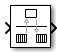
\includegraphics[width=0.5\textwidth]{imagenes/Rate Transition Block.png}
         \caption{Rate Transition \cite{RateTransition-MathWorks}}
         \label{fig:Rate Transition}
     \end{subfigure}
     \hfill
     \begin{subfigure}[b]{0.45\textwidth}
         \centering
         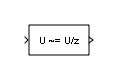
\includegraphics[width=0.5\textwidth]{imagenes/Detect Change Block.png}
         \caption{Detect Change \cite{DetectChange-Mathworks}}
         \label{fig:Detect Change}
     \end{subfigure}
        \caption{Bloques utilizados.}
        \label{fig:Bloques Subsistema Motores}
\end{figure}

La señal `\textit{Mode}' también será recibida por el bloque `\textit{Switch Case}' que detectará el modo de funcionamiento encauzando así la señal que queremos que se transmita a los motores. Estos comandos especiales se encuentran en el documento de Ben Katz \cite{Katz2021} y son:

\begin{itemize}
    \item \textit{Enter Motor Mode}: [0xFF, 0xFF, 0xFF, 0xFF, 0xFF, 0xFF, 0xFF, 0xFC]
    \item \textit{Exit Motor Mode}: [0xFF, 0xFF, 0xFF, 0xFF, 0xFF, 0xFF, 0xFF, 0xFD]
    \item \textit{Zero Position Sensor}: [0xFF, 0xFF, 0xFF, 0xFF, 0xFF, 0xFF, 0xFF, 0xFE]
\end{itemize}

El bloque `\textit{Merge}' se encargará de combinar las entradas en una única salida que será la entrada a los bloques `\textit{CAN Pack}' esta vez configurados seleccionando que `\textit{Data is input as}' es \textit{raw data}.

En esta parte también se realiza el empaquetado de los parámetros de control de cada motor. Se utilizan las entradas correspondientes a los vectores de cada motor, estos se pasan inicialmente por un bloque de `\textit{Data Type Conversion}' para asegurar que todos los componentes del vector son del tipo \textit{single}. Una vez hecho esto se sacan cada uno de los parámetros mediante el bloque `\textit{Demux}' y se conecta con el `\textit{CAN Pack}' con la configuración mostrada previamente en este capítulo de la memoria (Figura \ref{fig:Simulink-CANPack})

El valor negado proveniente del bloque `\textit{Detect Change}' será el que se utilice en los bloques `\textit{Switch}' para que la información que transmita finalmente a los motores sea el nuevo modo de funcionamiento o el control de estos. Se decide configurar que el bloque `\textit{CAN Transmit}' muestre su \textit{status} para poder visualizar durante las pruebas si se está produciendo un error en la trasmisión de datos. Añadiéndose junto a este, una captura de pantalla de la ayuda por parte de MathWorks para traducir este código de error fácilmente.

\begin{figure}[H]
    \centering
    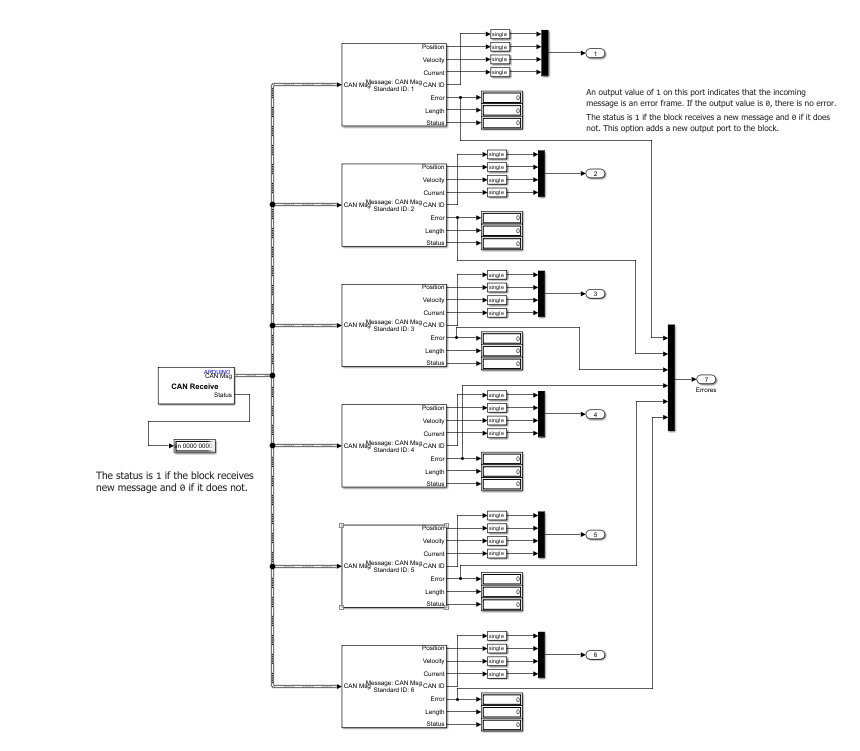
\includegraphics[width=\linewidth]{imagenes/Simulink - Cont - 2.png}
    \caption{Recepción de datos de los motores.}
    \label{fig:Simulink-Motores3}
\end{figure}

Esta última parte es la encargada del desempaquetado de los mensajes CAN recibidos por el Arduino. El bloque `\textit{CAN Receive}' al igual que el `\textit{CAN Transmit}' es configurado para que muestre su \textit{status}, esta vez para identificar si se está recibiendo un mensaje nuevo o no. Este bus se hace llegar a los diferentes bloques de de `\textit{CAN Unpack}' que se encuentran con la configuración mostrada previamente en la figura \ref{fig:Simulink-CANUnpack}.

Los parámetros recibidos se multiplexaran en un vector para cada motor y pasarán a la salida del subsistema. Estos bloques `\textit{CAN Unpack}' además mostrarán señales de error, longitud y estado. Que servirán para determinar si el mensaje se trata de una trama de error o no, y si se está recibiendo nueva información o no.

\section{Arduino MKR}

Previamente en esta memoria se propuso la utilización de una placa Arduino MKR y su respectiva \textit{shield}, que permitiese una posterior comunicación inalámbrica con el vehículo robótico. Se realiza por tanto un código básico (Anexo \ref{ComunicacionMotores.ino}) para probar la comunicación entre esta nueva placa y el motor. A continuación se describen las partes de interés del código.

\begin{lstlisting}[language=Arduino, caption= Definiciones Básicas, basicstyle=\scriptsize]
unsigned char Enter_Motor_Mode[8] = {0xFF, 0xFF, 0xFF, 0xFF, 0xFF, 0xFF, 0xFF, 0xFC};
unsigned char Exit_Motor_Mode[8] = {0xFF, 0xFF, 0xFF, 0xFF, 0xFF, 0xFF, 0xFF, 0xFD};

unsigned char buf;
unsigned char len = 0;
long unsigned int canID = 0;
unsigned char ID_type = 0;
\end{lstlisting}

En esta primera parte del código se inicializan las variables que vamos a utilizar posteriormente. \textit{Enter\_Motor\_Mode} y \textit{Exit\_Motor\_Mode} son las señales específicas del motor que hace que se enciendan y apaguen respectivamente. \cite{Katz2021} 

\begin{lstlisting}[language=Arduino, caption= Función Setup, basicstyle=\scriptsize]
void setup() {
  // put your setup code here, to run once:
  SERIAL.begin(115200);

  while(CAN_OK != CAN.begin(0 ,CAN_1000KBPS, MCP_16MHZ)) {
    SERIAL.println("CAN BUS Shield init fail!");
    SERIAL.println("Init CAN BUS Shield again");
    delay(10);
  }

  SERIAL.println("CAN BUS Shield init ok!");

  CAN.sendMsgBuf(0x05, 0, 8, Enter_Motor_Mode);

  delay(1000);

  // CAN.sendMsgBuf(0x05, 0, 8, Exit_Motor_Mode);

  // delay(1000);

}
\end{lstlisting}

En esta parte se recoge la configuración y se ejecutará una única vez. La función se encargará de inicializar la \textit{CAN Bus Shield} y de informarnos a través del monitor serie si se ha realizado correctamente o si ha fallado. Además se envía la señal de encendido de motores una vez 

\begin{lstlisting}[language=Arduino, caption= Función Loop, basicstyle=\scriptsize]
void loop() {
  // put your main code here, to run repeatedly:


  
  if(CAN_MSGAVAIL == CAN.checkReceive()){
    CAN.readMsgBuf(&canID, &ID_type, &len, &buf);
    SERIAL.println(len);
  
    SERIAL.println("----------------------");
    SERIAL.println("Get data from ID: 0x");
    SERIAL.println(canID, HEX);

    SERIAL.println(buf, HEX);
    SERIAL.println("\t");

    SERIAL.println();
  }

  else
    SERIAL.println("No llega nada");

  delay(1000);

}
\end{lstlisting}

Esta parte del código será la que se ejecute cíclicamente. En ella se comprueba la recepción de información a través del CAN. En caso de recibirse, imprime en el monitor serie la ID del motor del cuál se ha recibido el mensaje, y el mensaje cuestión. Todo esto se mostrará en formato hexadecimal. En caso de no recibir nada, se imprimirá en el monitor serie el mensaje `No llega nada' que nos permitirá identificar que algo está fallando en la recepción de información.

Tras varios intentos se detecta que a pesar de la correcta inicialización de la \textit{shield} de Arduino. La comunicación entre esta y el motor falla, puesto que al mandar la señal de encendido (\textit{Enter\_Motor\_Mode}) estos no lo hacen. Por tanto se decide seguir con la placa Arduino Mega.

%\blankpage